\chapter{Conclusion}
\label{chp:conclusions}
This desktop study was motivated by the consideration of sea level from within the Australian Bureau of Meteorology, and certain conceptual problems identified behind operational developments.
Exploration of the intersection of conventional tide prediction and operational mesoscale ocean forecasts within the agency has highlighted nuanced issues of representation, system compatibility and user expectation that are relevant to the strategic direction towards ``seamless'' services.
As such, all evaluations treated here have intentionally not pursued higher fidelity coastal simulations, but instead directed attention to some less-studied aspects of evaluating and exploiting predictability with established operational systems.   

As a thesis with publication, much of the body of this document has been published as, or is in preparation for peer-reviewed academic papers.
%------------------------
\section{Findings summary}
In answer to the research questions posed in \ref{Sec:intro} the findings of this thesis are summarises as follows:
Firstly, it was demonstrated that incompatible definitions of ocean ``tide'' are in parallel operational use.
Whereas downscaling for coastal sea level forecasts is clearly a productive approach, mesoscale ocean forecasts can immediately and directly provide significant but qualified forecast value for coastal sea level.
The fact that nominally tidal signals are present in mesoscale non-tidal ocean simulations means that care is required to avoid misinterpretation.

An aggregation approach that combines existing heterogeneous data but accounts for double-counting provides an important skill benchmark for future sea level forecast system development.
The point-based bias correction characteristics from these aggregated forecasts indicate that coastally contiguous extensions to model aggregation may be feasible.


In the operational context of combining and upgrading forecast models, it was shown that the coastal propagation characteristics of candidate forecast systems can be usefully evaluated and compared in a grid-independent waveguide projection.
Such a coastal waveguide projection also offers a means to direct forecaster attention to signals of special relevance along the Australian mainland coast.

Finally, it was argued that conventional harmonic tide predictions are not redundant, despite the ongoing advances in hydrodynamic simulation,  but that operational tide services require appropriate product differentiation to compliment modern applications and facilitate future refinement.
     % <<-- external file

%------------------------
\section{Heterogeneous simulations and seamless services}
The original coinage of "seamless" prediction in the context of climate projections has evolved to now encompass the more general goal of prediction across time and length scales \citep{10.1127/metz/2020/1048}.
Indeed the development of more seamless services is a strategic goal of the Australian Bureau of Meteorology \cite{BOM2020}.
\cite{10.1175/bams-89-4-459} illustrated the concept with a schematic chain of scales reaching from the small and fast out to the large and slow.
The present focus on sea level forecasting allows for a twist on the chain image to highlight the unusual place in which the LTI tidal admittance approach can be located relative to the geophysical fluid suite of simulations.
Figure \ref{fig:forecastScalesChain} schematically shows that tide prediction in general can provide very long horizon prognoses of short time scale fluctuations in sea level; of course subject to many caveats.
%------------------------------
\begin{figure}[H]\centering
        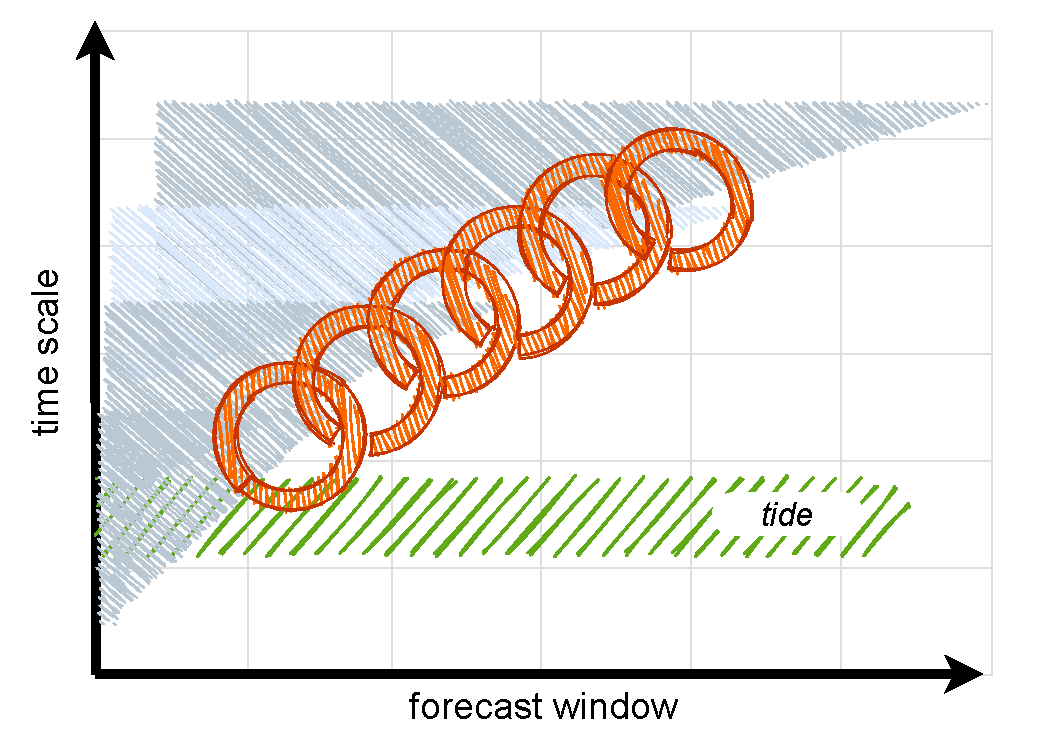
\includegraphics[width=\figwidthFull]{figures/diagrams/scales_with_chain.pdf} 
        \caption{Tide prediction can sit awkwardly with the seamless chain of scales analogy; following Figure \ref{fig:forecastScalesAll} and \citep{10.1175/bams-89-4-459}}
        \label{fig:forecastScalesChain}
\end{figure}
%------------------------------
The intention behind this picture is to emphasise that multi-scale prediction need not be shoe-horned into the tidy cascade of a single consistent earth system simulation framework.
Although the idea of a single simulation code-base and forecasting framework is attractive on many fronts  \footnote{\url{https://research.csiro.au/access/what/}}, consideration of the status of sea level and tide prediction provides at least one case in which some sort of exception is sure to be required based on the unique value offered by legacy products.  

Operational reality is expected to always consist to a some degree of a suite of systems that are not cleanly compatiable ....

Numerical forecasts from agencies like the Australian Bureau of Meteorology have arguably been under-utilised as a result of system heterogeneity.   It is not self-evident how to take into account the prognostic information ostensibly available in non-tidal sea level anomaly, storm surge and tide-table products; whereas all could be simultaneously issued to the public. 

.... some lessons for any blended information from climate, short term and long term forecasts for decision making is in 

%------------------------
\section{Next steps}
Australia ....versus OS.

Primacy of observational data and metadata

Expansion to more heterogenous and diverse quality data ...video etc


Seamless ...

Microservice architecture 
...foundational prediction systems 
...accessible and machine-readable 
...contrast to highly targeted vertical stack like ROAM   ...better to ensure value can be extracted and 

Historical legacy and user adapatation ...

All in the context of repairing whilst on 

Something about keeping up connection and dialogue with academic and cutting edge ....bluelink collaboration ...not just user pull ...




